% 声速测定实验报告。基于本目录“物理实验报告模板.tex”排版。
% 编译：xelatex 声速测定.tex（交叉引用需编译两次）。
% 后端填数：在下方“数据输入区”插入 \SetField{键}{值}；值可含 LaTeX 命令。
% 未设置的字段显示为空白横线。所有实验测量值、计算结果和个人信息均默认留空。
\documentclass[UTF8,a4paper,10pt,fontset=fandol]{ctexart}
\usepackage[left=3.175cm,right=3.175cm,top=2.54cm,bottom=2.54cm]{geometry}
\usepackage{graphicx}
\usepackage{tikz}
\usepackage{fancyhdr}
\usepackage{lastpage}
\usepackage{amsmath}
\usepackage{booktabs}
\usepackage{array}
\usepackage{needspace}

\setlength{\parindent}{0pt}
\setlength{\parskip}{0pt}
\setlength{\headheight}{18pt}
\linespread{1}

% 数据字段。Python 可在数据输入区写入：\SetField{res_l01}{30.40}
\newcommand{\SetField}[2]{\expandafter\def\csname expdata@#1\endcsname{#2}}
\newcommand{\Field}[2][1.7cm]{%
  \underline{\makebox[#1][c]{%
    \ifcsname expdata@#2\endcsname\csname expdata@#2\endcsname\else\strut\fi}}}
\newcommand{\MathField}[2][1.7cm]{\mbox{\Field[#1]{#2}}}
\newif\ifreportimages

% ===== 数据输入区开始 =====
\SetField{experiment}{声速测定}
% 示例：\SetField{student}{姓名}
% 示例：\SetField{res_l01}{30.40}
% 字段名见正文；res = 共振干涉法，phase = 相位比较法。
% ===== 数据输入区结束 =====

\newcommand{\coverfield}[2]{%
  \noindent{\heiti\fontsize{18pt}{48pt}\selectfont
  \makebox[3.3cm][l]{#1}\Field[8.8cm]{#2}\par}%
}

% 沿用报告模板的装订线。
\newcommand{\bindingline}[1][2.85]{%
  \begin{tikzpicture}[remember picture,overlay]
    \foreach \i in {0,...,38}{%
      \pgfmathsetmacro{\bindingy}{-#1-0.52*\i}%
      \ifnum\i=13\relax
        \node[inner sep=0pt] at
          ([xshift=1.05cm,yshift=\bindingy cm]current page.north west)
          {\songti\fontsize{10.5pt}{10.5pt}\selectfont 装};
      \else\ifnum\i=19\relax
        \node[inner sep=0pt] at
          ([xshift=1.05cm,yshift=\bindingy cm]current page.north west)
          {\songti\fontsize{10.5pt}{10.5pt}\selectfont 订};
      \else\ifnum\i=25\relax
        \node[inner sep=0pt] at
          ([xshift=1.05cm,yshift=\bindingy cm]current page.north west)
          {\songti\fontsize{10.5pt}{10.5pt}\selectfont 线};
      \else
        \pgfmathsetmacro{\bindingtop}{\bindingy+0.20}%
        \pgfmathsetmacro{\bindingbottom}{\bindingy-0.20}%
        \draw[line width=0.35pt,dash pattern=on 1.2pt off 1.8pt]
          ([xshift=1.05cm,yshift=\bindingtop cm]current page.north west)
          -- ([xshift=1.05cm,yshift=\bindingbottom cm]current page.north west);
      \fi\fi\fi
    }
  \end{tikzpicture}%
}

\fancypagestyle{report}{%
  \fancyhf{}
  \fancyhead[C]{}
  \fancyfoot[C]{第\thepage 页\quad 共\pageref{LastPage}页}
  \renewcommand{\headrulewidth}{0.4pt}
  \renewcommand{\footrulewidth}{0pt}
}
\fancypagestyle{record}{%
  \fancyhf{}
  \fancyhead[C]{原始数据记录单}
  \fancyfoot[C]{第\thepage 页\quad 共\pageref{LastPage}页}
  \renewcommand{\headrulewidth}{0.4pt}
  \renewcommand{\footrulewidth}{0pt}
}

\newcommand{\reportsection}[1]{\par\Needspace{4\baselineskip}\vspace{0.7\baselineskip}{\heiti #1}\par\vspace{0.15\baselineskip}}
\newcommand{\reportsubsection}[1]{\par\Needspace{3\baselineskip}\vspace{0.35\baselineskip}{\heiti #1}\par}

\begin{document}
\fontsize{10.5pt}{18pt}\selectfont

% 第 1 页：封面
\thispagestyle{empty}
\vspace*{1.0cm}
\begin{center}
  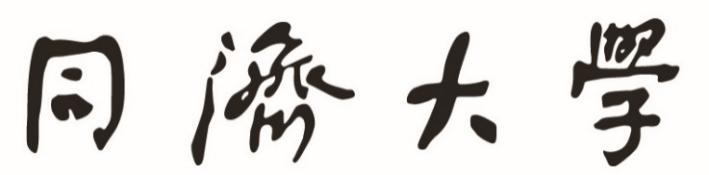
\includegraphics[width=8.184cm]{tongji_logo.jpeg}\par
  {\bfseries\fontsize{18pt}{24pt}\selectfont TONGJI UNIVERSITY\par}
  \vspace{1.5cm}
  {\heiti\fontsize{36pt}{44pt}\selectfont 物理实验报告\par}
\end{center}
\vspace{1.5cm}
\coverfield{实验名称}{experiment}
\coverfield{学生姓名}{student}
\coverfield{学\hspace{1em}号}{student_id}
\coverfield{组\hspace{1em}号}{group}
\coverfield{实验日期}{date}

\clearpage
\pagestyle{report}
\bindingline
\begin{center}
  {\heiti\fontsize{14pt}{30pt}\selectfont 声速测定\par}
\end{center}

\reportsection{实验目的}
1. 了解压电换能器的原理与功能。\par
2. 掌握用示波器观察驻波及振动合成实验现象。\par
3. 掌握用共振干涉法与相位比较法测定波长。\par
4. 测定室温下空气中的声速。\par
5. 培养综合使用仪器的能力。\par
6. 练习用逐差法处理实验数据。\par

\reportsection{实验原理}
声音传播的行为与传播介质相关，通常受以下三个因素影响：\par
1. 介质的密度与压力。受温度影响的这种关系决定了介质中声音的速度。\par
2. 声波传播也受到介质本身运动的影响。如果介质正在移动，则声速随之改变。\par
3. 介质的黏度也会影响声波的运动，它决定声音衰减的速率。对于许多介质，例如空气或水，由于黏度引起的衰减可以忽略不计。本次实验介质为空气，其造成的衰减忽略不计。\par
通常有两种方式测定声速。一种是根据位移与速度关系，测出声波传播路程 $L$ 所需的时间 $t$，进而计算声速 $v=L/t$；这也是在实际工程中应用最广泛的一种方法。另一种是根据频率 $f$ 和波长 $\lambda$ 计算：
\begin{equation*}
  v=f\lambda .
\end{equation*}
本实验使用后一种方法，分别通过共振干涉法（驻波法）与相位比较法确定波长。相邻幅度极大位置或相邻同相位直线位置的间距均为半波长。连续测量 20 个位置后，按原文的逐差关系计算：
\begin{equation*}
  \lambda_i=\frac{l_{i+10}-l_i}{5},\qquad i=1,\ldots,10.
\end{equation*}
以平均室温 $\bar t$（摄氏度）估算干燥空气中的理论声速：$v_{\mathrm{th}}=331\sqrt{1+\bar t/273}\,\mathrm{m/s}$。\par

\reportsection{实验内容}
\reportsubsection{预备实验：数字示波器观测相位差}
1. 调整示波器，显示合适的信号波形。\par
2. 观察并绘制相位差为 $0^\circ$、$90^\circ$、$180^\circ$、$270^\circ$、$360^\circ$ 时的李萨如图形。\par

\reportsubsection{共振干涉法}
1. 调整实验装置：将压电陶瓷换能器 $S_1$ 信号端口与低频信号发生器输出相连接，$S_2$ 信号端口连接至示波器 CH1 通道输入端。将 $S_2$ 移至 $S_1$ 附近，两者尽量靠近但不能相互接触，并调整两个端面平行。打开示波器和低频信号发生器，将后者频率设为 $35.0\,\mathrm{kHz}$。\par
2. 缓慢调整信号发生器频率，同时观察示波器显示的 $S_2$ 输出信号；当幅度达到最大值时，信号频率与压电换能器的固有频率匹配。\par
3. 缓慢右移 $S_2$，逐渐远离 $S_1$，同时观察示波器显示的信号幅度变化。用游标卡尺读出信号幅度极大值对应的 $S_2$ 位置 $l_i$，继续移动 $S_2$，连续读出 20 个相邻的幅度极大位置，再用逐差法计算波长。\par

\reportsubsection{相位比较法}
1. 将信号发生器的输出分别接 $S_1$ 和示波器 CH2 通道，将 $S_2$ 信号端口接示波器 CH1 通道。把示波器显示模式调为 X--Y，并按上述方法调整频率与换能器固有频率匹配。\par
2. 缓慢右移 $S_2$，逐渐远离 $S_1$。当示波器显示的李萨如图形为一特定角度的直线时，记录 $S_2$ 的位置 $l_i$；继续移动 $S_2$，连续读出 20 个相邻的直线位置，再用逐差法计算波长。\par

\reportsection{实验仪器}
低频信号发生器、数字示波器、声速测定装置（含游标卡尺）。\par

\reportsection{数据记录处理}
\reportsubsection{共振干涉法}
开始时室温 $t_1=\MathField[1.2cm]{res_t_start}\,{}^\circ\mathrm C$，结束时室温 $t_2=\MathField[1.2cm]{res_t_end}\,{}^\circ\mathrm C$，平均室温 $\bar t=\MathField[1.2cm]{res_t_avg}\,{}^\circ\mathrm C$。\par
信号频率 $f=\MathField[1.5cm]{res_frequency}\,\mathrm{kHz}$，频率误差 $\Delta_f=\MathField[1.4cm]{res_frequency_error}\,\mathrm{kHz}$。\par
\begin{center}
\small
\renewcommand{\arraystretch}{1.2}
\begin{tabular}{c c c c}
\toprule
$i$ & $l_i/\mathrm{mm}$ & $l_{i+10}/\mathrm{mm}$ & $\lambda_i=(l_{i+10}-l_i)/5\;/\mathrm{mm}$\\
\midrule
1  & \Field[1.35cm]{res_l01} & \Field[1.35cm]{res_l11} & \Field[1.35cm]{res_lambda01}\\
2  & \Field[1.35cm]{res_l02} & \Field[1.35cm]{res_l12} & \Field[1.35cm]{res_lambda02}\\
3  & \Field[1.35cm]{res_l03} & \Field[1.35cm]{res_l13} & \Field[1.35cm]{res_lambda03}\\
4  & \Field[1.35cm]{res_l04} & \Field[1.35cm]{res_l14} & \Field[1.35cm]{res_lambda04}\\
5  & \Field[1.35cm]{res_l05} & \Field[1.35cm]{res_l15} & \Field[1.35cm]{res_lambda05}\\
6  & \Field[1.35cm]{res_l06} & \Field[1.35cm]{res_l16} & \Field[1.35cm]{res_lambda06}\\
7  & \Field[1.35cm]{res_l07} & \Field[1.35cm]{res_l17} & \Field[1.35cm]{res_lambda07}\\
8  & \Field[1.35cm]{res_l08} & \Field[1.35cm]{res_l18} & \Field[1.35cm]{res_lambda08}\\
9  & \Field[1.35cm]{res_l09} & \Field[1.35cm]{res_l19} & \Field[1.35cm]{res_lambda09}\\
10 & \Field[1.35cm]{res_l10} & \Field[1.35cm]{res_l20} & \Field[1.35cm]{res_lambda10}\\
\bottomrule
\end{tabular}
\end{center}
平均波长 $\bar\lambda=\MathField[1.5cm]{res_lambda_avg}\,\mathrm{mm}$；不确定度按下式计算。
\begin{align*}
U_{A,\lambda}&=\sqrt{\frac{\sum_{i=1}^{n}(\lambda_i-\bar\lambda)^2}{n(n-1)}}
  =\MathField[1.4cm]{res_u_a}\,\mathrm{mm},\\
U_{B,\lambda}&=\frac{\Delta_l}{\sqrt3}=\MathField[1.4cm]{res_u_b}\,\mathrm{mm},\\
U_\lambda&=\sqrt{U_{A,\lambda}^2+U_{B,\lambda}^2}
  =\MathField[1.4cm]{res_u_lambda}\,\mathrm{mm},\qquad
U_{r\lambda}=\frac{U_\lambda}{\bar\lambda}
  =\MathField[1.4cm]{res_u_r_lambda},\\
U_f&=\frac{\Delta_f}{\sqrt3}=\MathField[1.4cm]{res_u_f}\,\mathrm{kHz},\qquad
U_{rf}=\frac{U_f}{f}=\MathField[1.4cm]{res_u_r_f},\\
v&=\bar\lambda f=\MathField[1.5cm]{res_speed}\,\mathrm{m/s},\\
U_{rv}&=\sqrt{\left(\frac{U_\lambda}{\bar\lambda}\right)^2+
              \left(\frac{U_f}{f}\right)^2}
  =\MathField[1.4cm]{res_u_r_v},\qquad
U_v=U_{rv}v=\MathField[1.4cm]{res_u_v}\,\mathrm{m/s}.
\end{align*}
\Needspace{5\baselineskip}
实验结果：$v=(\MathField[1.5cm]{res_speed_result}\pm\MathField[1.2cm]{res_u_v_result})\,\mathrm{m/s}$。相对不确定度 $U_{rv}=\MathField[1.2cm]{res_u_r_v_percent}\%$。与理论值 $v_{\mathrm{th}}=\MathField[1.5cm]{res_speed_theory}\,\mathrm{m/s}$ 比较，百分差
\begin{equation*}
E=\frac{|v-v_{\mathrm{th}}|}{v_{\mathrm{th}}}\times100\%
 =\MathField[1.2cm]{res_error_percent}\%.
\end{equation*}

\reportsubsection{相位比较法}
开始时室温 $t_1=\MathField[1.2cm]{phase_t_start}\,{}^\circ\mathrm C$，结束时室温 $t_2=\MathField[1.2cm]{phase_t_end}\,{}^\circ\mathrm C$，平均室温 $\bar t=\MathField[1.2cm]{phase_t_avg}\,{}^\circ\mathrm C$。\par
信号频率 $f=\MathField[1.5cm]{phase_frequency}\,\mathrm{kHz}$，频率误差 $\Delta_f=\MathField[1.4cm]{phase_frequency_error}\,\mathrm{kHz}$。\par
\begin{center}
\small
\renewcommand{\arraystretch}{1.2}
\begin{tabular}{c c c c}
\toprule
$i$ & $l_i/\mathrm{mm}$ & $l_{i+10}/\mathrm{mm}$ & $\lambda_i=(l_{i+10}-l_i)/5\;/\mathrm{mm}$\\
\midrule
1  & \Field[1.35cm]{phase_l01} & \Field[1.35cm]{phase_l11} & \Field[1.35cm]{phase_lambda01}\\
2  & \Field[1.35cm]{phase_l02} & \Field[1.35cm]{phase_l12} & \Field[1.35cm]{phase_lambda02}\\
3  & \Field[1.35cm]{phase_l03} & \Field[1.35cm]{phase_l13} & \Field[1.35cm]{phase_lambda03}\\
4  & \Field[1.35cm]{phase_l04} & \Field[1.35cm]{phase_l14} & \Field[1.35cm]{phase_lambda04}\\
5  & \Field[1.35cm]{phase_l05} & \Field[1.35cm]{phase_l15} & \Field[1.35cm]{phase_lambda05}\\
6  & \Field[1.35cm]{phase_l06} & \Field[1.35cm]{phase_l16} & \Field[1.35cm]{phase_lambda06}\\
7  & \Field[1.35cm]{phase_l07} & \Field[1.35cm]{phase_l17} & \Field[1.35cm]{phase_lambda07}\\
8  & \Field[1.35cm]{phase_l08} & \Field[1.35cm]{phase_l18} & \Field[1.35cm]{phase_lambda08}\\
9  & \Field[1.35cm]{phase_l09} & \Field[1.35cm]{phase_l19} & \Field[1.35cm]{phase_lambda09}\\
10 & \Field[1.35cm]{phase_l10} & \Field[1.35cm]{phase_l20} & \Field[1.35cm]{phase_lambda10}\\
\bottomrule
\end{tabular}
\end{center}
平均波长 $\bar\lambda=\MathField[1.5cm]{phase_lambda_avg}\,\mathrm{mm}$。\par
\begin{align*}
U_{A,\lambda}&=\sqrt{\frac{\sum_{i=1}^{n}(\lambda_i-\bar\lambda)^2}{n(n-1)}}
  =\MathField[1.4cm]{phase_u_a}\,\mathrm{mm},\\
U_{B,\lambda}&=\frac{\Delta_l}{\sqrt3}=\MathField[1.4cm]{phase_u_b}\,\mathrm{mm},\\
U_\lambda&=\sqrt{U_{A,\lambda}^2+U_{B,\lambda}^2}
  =\MathField[1.4cm]{phase_u_lambda}\,\mathrm{mm},\qquad
U_{r\lambda}=\frac{U_\lambda}{\bar\lambda}
  =\MathField[1.4cm]{phase_u_r_lambda},\\
U_f&=\frac{\Delta_f}{\sqrt3}=\MathField[1.4cm]{phase_u_f}\,\mathrm{kHz},\qquad
U_{rf}=\frac{U_f}{f}=\MathField[1.4cm]{phase_u_r_f},\\
v&=\bar\lambda f=\MathField[1.5cm]{phase_speed}\,\mathrm{m/s},\\
U_{rv}&=\sqrt{\left(\frac{U_\lambda}{\bar\lambda}\right)^2+
              \left(\frac{U_f}{f}\right)^2}
  =\MathField[1.4cm]{phase_u_r_v},\qquad
U_v=U_{rv}v=\MathField[1.4cm]{phase_u_v}\,\mathrm{m/s}.
\end{align*}
\Needspace{5\baselineskip}
实验结果：$v=(\MathField[1.5cm]{phase_speed_result}\pm\MathField[1.2cm]{phase_u_v_result})\,\mathrm{m/s}$。相对不确定度 $U_{rv}=\MathField[1.2cm]{phase_u_r_v_percent}\%$。与理论值 $v_{\mathrm{th}}=\MathField[1.5cm]{phase_speed_theory}\,\mathrm{m/s}$ 比较，百分差
\begin{equation*}
E=\frac{|v-v_{\mathrm{th}}|}{v_{\mathrm{th}}}\times100\%
 =\MathField[1.2cm]{phase_error_percent}\%.
\end{equation*}

\reportsection{讨论与分析}
\reportsubsection{两种测量方法的对比}
共振干涉法利用 $S_1$ 发射声波，$S_2$ 接收并反射，在两者之间形成驻波。移动 $S_2$ 并观察示波器上信号幅度的极大值，可确定对应位置。该方法物理图像直观，但极值点的判断会受到环境噪声和信号源幅度波动的影响。\par
相位比较法将发射信号和接收信号分别输入示波器的两个通道。当两者相位差为 $0$ 或 $\pi$ 时，合成轨迹为直线。通过观察直线出现的位置确定波长；图形变化有助于判断相位状态。\par
\reportsubsection{误差来源与改进}
游标卡尺的仪器误差 $\Delta_l=\MathField[1.2cm]{caliper_error}\,\mathrm{mm}$、信号发生器的频率漂移及示波器分辨率，均可能影响测量结果。实验中应保持室温稳定，避免实验台振动，并仔细调整换能器的共轴和平行状态。可使用数显测距与自动采集、示波器光标或计算机峰值捕捉，以减少人为读数和极值判断误差。\par
本次测量两种方法得到的声速相差 $\MathField[1.5cm]{method_difference}\,\mathrm{m/s}$。与各自室温下的理论值相比，\Field[3.0cm]{closer_method}的百分差较小。两法所得结果不完全一致，主要因为共振峰位置及李萨如图形成为直线的时刻需要人工判断；换能器端面不平行、环境温度变化和频率漂移也会引入系统误差。\par
\reportsubsection{思考题}
为何采用逐差法？将相隔 10 个位置的读数作差，可利用较长的测量距离求波长，减弱单次位置读数误差的影响；再对 10 组结果取平均，可降低随机误差。\par
为何在两种方法中均需调节信号频率？使激励频率接近换能器固有频率，接收信号更明显，有利于辨认幅度极大和相位对应位置。\par
温度为何必须记录？空气中的声速随温度变化；记录起止温度并取平均，才能计算与测量过程对应的理论值，合理比较百分差。\par

\reportsection{实验结论}
本实验利用共振干涉法和相位比较法测定空气中的声速，并用逐差法处理多组位置数据。\par
\begin{center}
\small
\renewcommand{\arraystretch}{1.25}
\begin{tabular}{l c c c c c c}
\toprule
方法 & $f/\mathrm{kHz}$ & $\bar t/{}^\circ\mathrm C$ & $\bar\lambda/\mathrm{mm}$ & $v/(\mathrm{m/s})$ & $U_{rv}/\%$ & $E/\%$\\
\midrule
共振干涉法 & \Field[1.1cm]{res_frequency} & \Field[1.1cm]{res_t_avg} & \Field[1.1cm]{res_lambda_avg} & \Field[1.1cm]{res_speed_result} & \Field[0.9cm]{res_u_r_v_percent} & \Field[0.9cm]{res_error_percent}\\
相位比较法 & \Field[1.1cm]{phase_frequency} & \Field[1.1cm]{phase_t_avg} & \Field[1.1cm]{phase_lambda_avg} & \Field[1.1cm]{phase_speed_result} & \Field[0.9cm]{phase_u_r_v_percent} & \Field[0.9cm]{phase_error_percent}\\
\bottomrule
\end{tabular}
\end{center}
取两种方法结果的算术平均，本实验测得当前室温下空气中的声速约为 $\MathField[1.5cm]{final_speed}\,\mathrm{m/s}$。\par

\clearpage
\thispagestyle{record}
\bindingline[3.03]
\vspace*{0.6cm}
\ifreportimages\else（请将教师签字的实验原始数据记录单完整拍照并粘贴于此。）\fi

% ===== 原始数据图片插入区 =====

\end{document}
